\chapter{Matching Methods}
Basically c/p from paper, but better figures and maybe more explanations
 - Add path about graphs and how they are formed. Make sure to explain 
 the clustering in more detail and make it easier to understand
 - Add a good explanation for new figures and how the precision and 
 recall are calculated. This should appear somewhere before results.
 - Add part on spectral matching and modify accordingly. Make sure to 
 underline how the second plot shows how the geometric method is 
 independent of MMC and that they combined yield greater results.

\subsection{Proposed Matching Methods}
\label{S:MatchingMethods}

\subsubsection{Mirror Match (\emph{MM})}

\begin{figure}[h]
	\centering%
		\begin{subfigure}[t]{0.5\columnwidth}
			\centering
			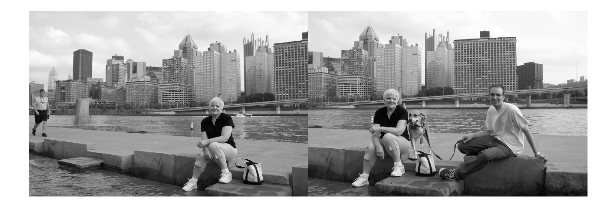
\includegraphics[width=0.95\columnwidth]{images/MMC_pitts_source}
			\caption{Source image pair}
			\label{fig:pitts_source}
		\end{subfigure}%
		~ %
		\begin{subfigure}[t]{0.5\columnwidth}
			\centering
			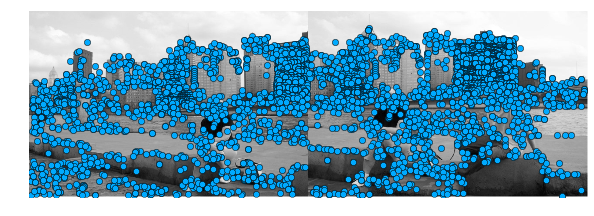
\includegraphics[width=0.95\columnwidth]{images/MMC_pitts_keypoints}
			\caption{Feature points}
			\label{fig:pitts_keypoints}
		\end{subfigure}%
		\\ %add desired spacing between images, e. g. ~, \quad, 
		%\qquad (or a blank line to force the subfigure onto a new line)
		\begin{subfigure}[t]{0.5\columnwidth}
			\centering
			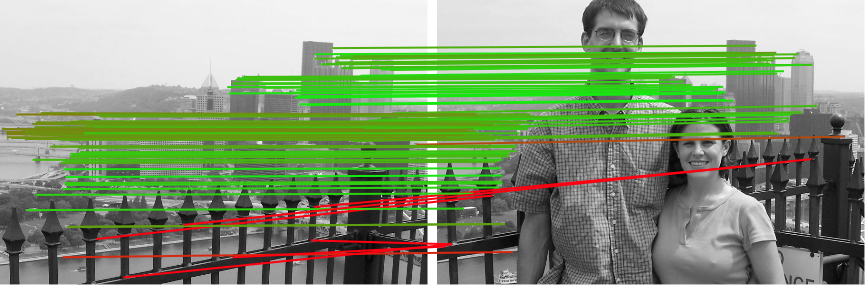
\includegraphics[width=0.95\columnwidth]{images/mirror_match_off}
			\caption{\emph{Ratio}}
			\label{fig:unique}
		\end{subfigure}%
		~ %add desired spacing between images, e. g. ~, \quad, 
		\begin{subfigure}[t]{0.5\columnwidth}
			\centering
			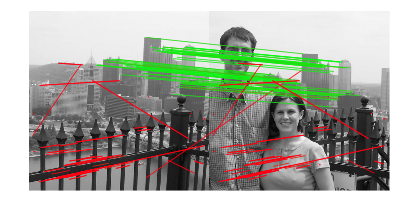
\includegraphics[width=0.95\columnwidth]{images/mirror_match_with_pruned}
			\caption{\emph{MM} intermediate result}
			\label{fig:within}
		\end{subfigure}%
		\\ %add desired spacing between images, e. g. ~, \quad, 
		%\qquad (or a blank line to force the subfigure onto a new line)
		\begin{subfigure}[t]{0.5\columnwidth}
			\centering
			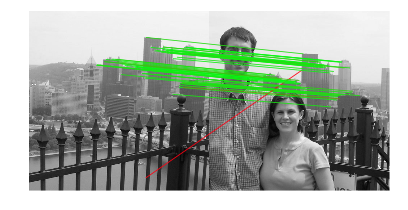
\includegraphics[width=0.95\columnwidth]{images/mirror_match}
			\caption{\emph{MM} final result}
			\label{fig:without}
		\end{subfigure}%
		~ %add desired spacing between images, e. g. ~, \quad, 
		\begin{subfigure}[t]{0.5\columnwidth}
			\centering
			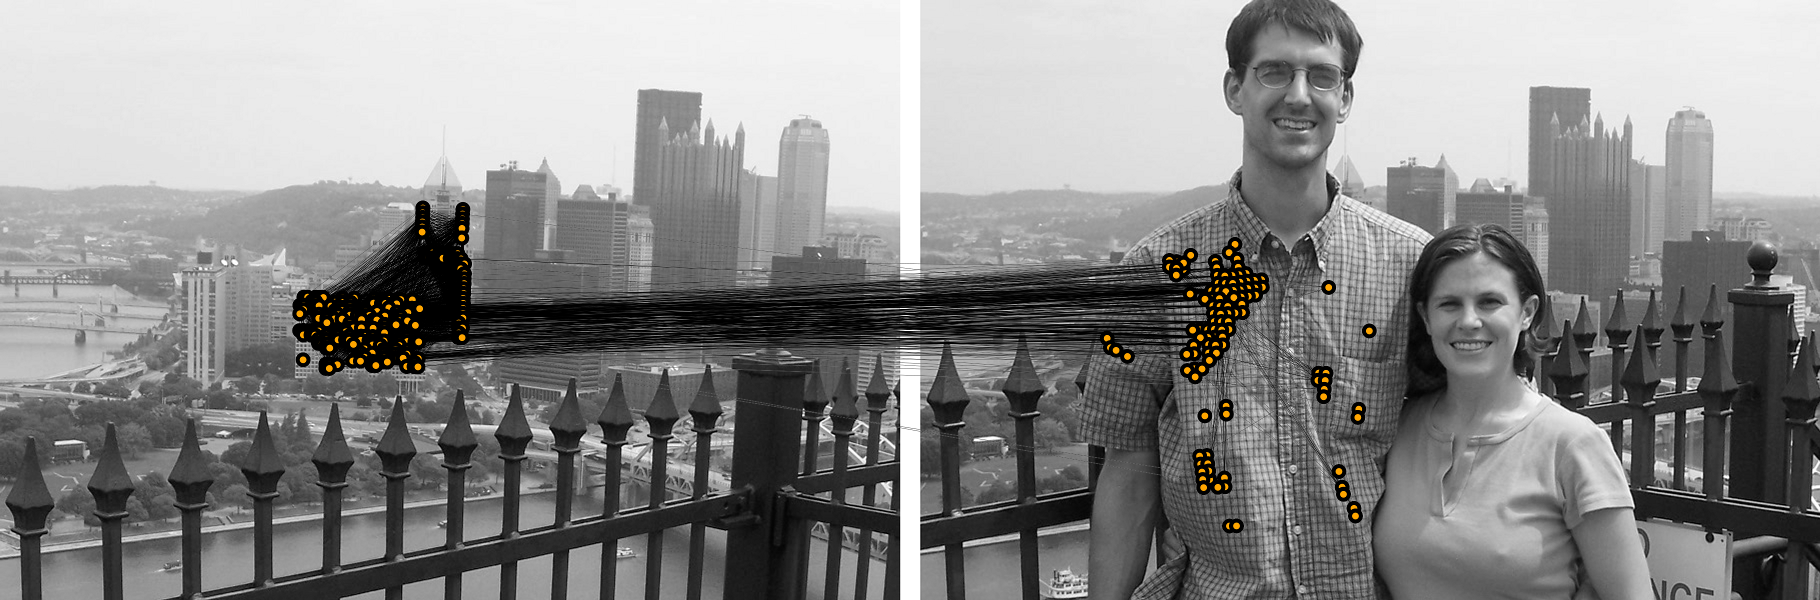
\includegraphics[width=0.95\columnwidth]{images/MMC_partition}
			\caption{\emph{MMC} Partition Example}
			\label{fig:pitts_partition}
		\end{subfigure}%
	\caption{Feature matching with \emph{MM} and \emph{MMC}. Dots represent feature points; green/red lines indicate correct/incorrect matches, respectively; black lines represent edges in the feature graph.  
	(c) Result of \emph{Ratio} matching. 
  (d) All matches found by \emph{MM}, including intra-image matches. 
	(e) Final \emph{MM} result. 
	(f) Example of a partition of feature points after clustering, which 
includes similar feature points from building windows and shirt patterns.}%
	\label{fig:comparemirror}%
\end{figure}%


%
The central idea behind \emph{MM} is to match features of $n$ images by 
taking every feature from all $n$ images and matching it against every 
other feature from the same set. We can then discard the correspondences 
that match two points within the same image. Algorithm~\ref{alg-mm} details  
the implementation of \emph{MM}.
%
\begin{algorithm}[h]
\caption{Mirror Match (\emph{MM})}
\label{alg-mm}
%{\fontsize{10}{10}\selectfont
\begin{algorithmic}
\Require $images$ : set of images, $t \in \mathbb{R}$
\State $matches_{init}\gets \varnothing$
\State $matches_{final}\gets \varnothing$
\State $features\gets \varnothing$
\ForAll{$I_i \in images$} \Comment Acquisition Stage
	\State $features\gets features \cup getFeatures(I_i)$
\EndFor
\ForAll{$f_i \in features$} \Comment Matching Stage
	\State $f_m,f_n \gets get2NNs(f_i, features \setminus 
	\left\{f_i\right\})$
	\State $ratio \gets similarity(f_i, f_n) / similarity(f_i, f_m)$
	\If{$ratio < t$}
		\State $matches_{init} \gets matches_{init} \cup \left(f_i, f_m\right)$
	\EndIf
\EndFor
\ForAll{$\left(f_i, f_j \right) \in matches_{init}$} \Comment Filter 
Stage
\If{$\left(f_j, f_i \right) \in matches_{init} \wedge getImg(f_i) \neq 
getImg(f_j) \wedge \left(f_j, f_i\right) \not\in matches_{final}$}
		\State $matches_{final} \gets (f_i, f_j)$
	\EndIf
\EndFor \\
\Return $matches_{final}$
\end{algorithmic}
%}
\end{algorithm}
%
In the acquisition stage we gather all features in the set of images.  
In the matching stage these features are matched using $k$-nearest 
neighbors.  For any given feature $f_i$ the two most similar neighbors 
are returned, and we calculate the ratio between them as proposed in 
\cite{lowe2004sift}.  Any correspondence with a ratio above the 
threshold supplied will be discarded. Finally in the filter stage we 
check that matches are from different images and discard all matches 
that are not symmetric.

Figure~\ref{fig:comparemirror} illustrates the benefits of \emph{MM} 
using an example image pair from the Gallagher dataset 
\cite{gallagher2008}.
With \emph{Ratio} (Figure~\ref{fig:unique}), many incorrect matches occur 
in the fence towards the bottom of the image.
When we match all feature points together, many of these incorrect 
matches are eliminated, because points in the fence match with other 
points in the fence in the same image (Figures~\ref{fig:within} and
\ref{fig:without}).


\subsubsection{Mirror Match with Clustering (\emph{MMC})}
%
In contrast to \emph{MM}, \emph{MMC} diverges from traditional 
non-geometric feature matching by clustering feature points by 
similarity. This process yields partitions of fairly similar feature 
points that we can match using the same approach as \emph{MM}.  
Algorithm~\ref{alg-mmc} shows the pseudocode implementation of \emph{MMC}.

Before we introduce the implementation details we will go over the 
problem of graph clustering and how it relates to feature matching.

Given a set of feature points from two images, $im_1$ and $im_2$: $F_k = 
\{k_i, k_j$ for $k_i \in im_1, k_j \in im_2\}$ as well as a matching 
function $M(k_i, k_j) \rightarrow \mathbb{R}$ that takes two feature 
points in an image and returns their matching score, we can define a 
matrix $A$ where each element $A_ij = M(k_i, k_j)$. A can be interpreted 
as the \emph{adjecency matrix} of the fully connected graph where each 
vertex corresponds to a keypoint and the edge between two vertices has a 
weight equal to the distance between the two corresponding keypoints.

This representation reduces the problem of partitioning the keypoints 
into groups to that of graph clustering or community structure depending 
on the context. In the literature there are various ways of clustering a 
graph according to different measures of what constitutes an optimal 
partitioning. Traditionally the most used clustering algorithms have 
been K-means and spectral clustering, but in recent years a host of new 
algorithms have been proposed based on both Newman's concept of graph 
modularity\footnote{Introduced in \cite{girvan2002}, discussed in 
\cite{brandes2007} and used in \cite{blondel2008} as well as others} as 
well as information theoretical measures\footnote{See for example 
\cite{rosvall2008}} and the Potts spin model from physics\footnote{Used 
in \cite{ronhovde2009}} just to mention a few approaches. Many of the 
new algorithms differ from K-means clustering and Spectral clustering 
in that they do not require the number of expected to clusters to be 
specified beforehand\footnote{Among the aforementioned methods, this is 
true for \cite{blondel2008} and \cite{rosvall2008}}.  Furthermore, on 
tests done using randomly generated graphs with a known partitioning 
\cite{blondel2008}, \cite{rosvall2008} and \cite{ronhovde2009} perform 
markedly better than spectral clustering and 
K-means\cite{lancichinetti2009}.

\begin{algorithm}[h]
\caption{Mirror Match with Clustering (\emph{MMC})}
\label{alg-mmc}
%{\fontsize{10}{10}\selectfont
\begin{algorithmic}
\Require $images$ : set of images, $t \in \mathbb{R}$
\State $M\gets \varnothing$
\State $F\gets \varnothing$
\ForAll{$I_i \in images$} \Comment Gather features
	\State $f_i\gets getFeatures(I_i)$
	\State $F\gets F \cup f_i$
\EndFor
\State $A\gets getAdjacencyMatrix(f_1, f_2,\; \ldots \;, f_n)$
\State $A_{norm}\gets 1 - normalize(A)$
\State $A_{pruned}\gets pruneEdges(A_{norm},\alpha)$
\State $P\gets cluster(A_{pruned})$
\ForAll{$p \in P$} \Comment p is a set of feature points
	\State $M\gets M \cup getMatches(p, t, F)$
\EndFor \\
\Return matches
\end{algorithmic}
%}
\end{algorithm}

The performance of clustering algorithms is a complicated issue, since 
an optimal clustering given the same graph can vary depending on the 
application. Spectral clustering for example will usually return a 
partitioning where each partition is roughly equal in size\footnote{As 
mentioned in \cite{von2007}} while the Louvain 
clustering\cite{blondel2008} might return partitions of very uneven 
size, even if the modularity measurement has been shown to penalize very 
small clusters\cite{brandes2007}. Both behaviours can be beneficial 
depending on the application, but when clustering feature points, 
maintaining clusters of an even size usually means that some clusters 
will be '\emph{catch-all}' clusters where the feature points that do 
not fit anywhere else are grouped together. The necessity of specifying 
the amount of partitions in for example Spectral clustering or Pott's 
model clustering further exacerbates the issue since smaller partitions 
are then combined into one to achieve the right amount of partitions.



\begin{figure}[t]
    \centering
	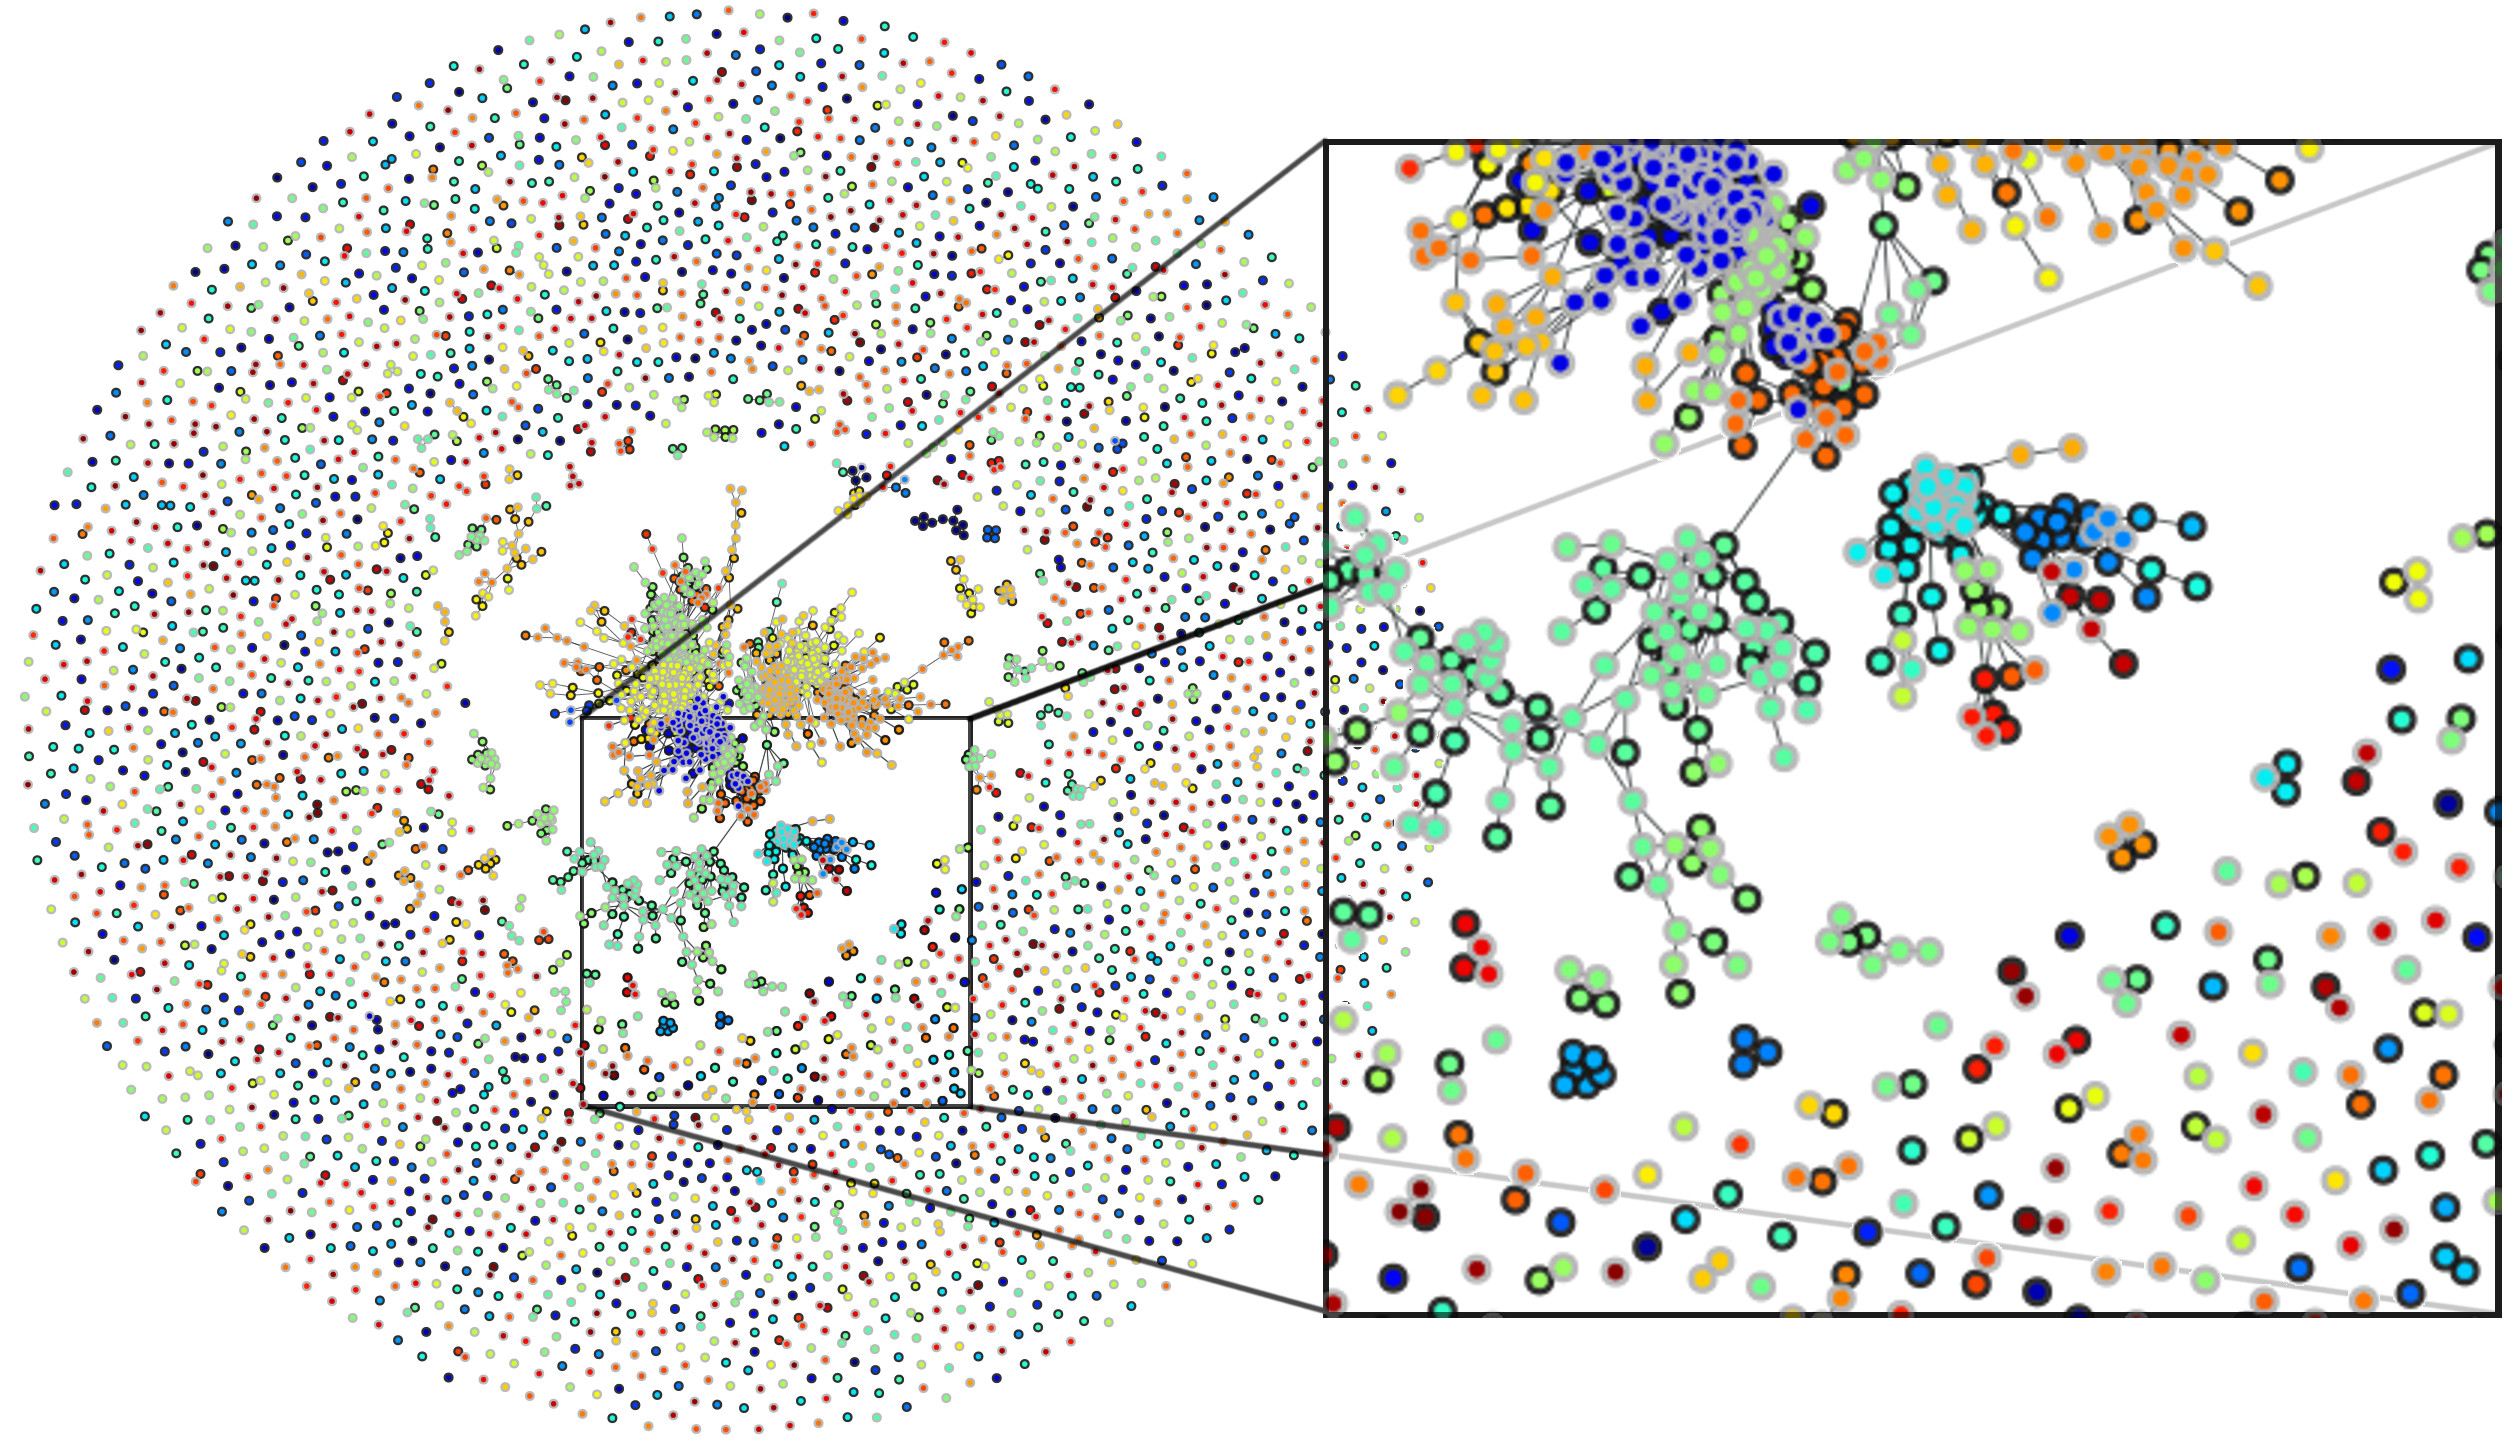
\includegraphics[width=\textwidth]{images/MMC_graph}
    \label{fig:graph}
	\caption{The partitioned feature graph. Each vertex represents a 
		feature point; lines indicate high similarity between points. A 
		partition is a connected group with the same color. The border 
		color of each node indicates which image it belongs to.  Zooming 
	into a subsection of the graph (right part), the various cluster 
sizes can be seen, ranging from hundreds of feature points to only two 
or three.}
	\label{fig:graph}
\end{figure}

We use the Louvain Method \cite{blondel2008} for clustering feature 
points, since it is relatively fast and performs well 
\cite{lancichinetti2009}, does not require parameters 
\cite{blondel2008}, and does not emphasize partitions of equal size, as 
opposed to spectral clustering or k-means \cite{von2007}, for example.
While the Louvain clustering algorithm does not require any parameters 
in itself, it tends towards clustering all feature points together in 
the same partition if the graph is very connected.  To ensure that the 
graph is well clustered, the adjacency matrix is pruned so that only 
edges above a certain threshold are kept. From empirical analysis, 
retaining the top 2.5\% of edges with the highest similarity seems to 
work well in practice. Figure~\ref{fig:graph} shows the result of 
clustering the feature points as a graph.
%

The partitions group feature points by similarity, which means that 
repetitive structures such as buildings often appear in larger 
partitions, as exemplified in Figure~\ref{fig:pitts_partition}.
%

\begin{algorithm}[h]
\caption{Impl.\ of getMatches (\emph{from MMC algorithm})}
\label{alg-getmatches}
    \fontsize{10}{10}\selectfont
    \begin{algorithmic}
    \Require $p$ : set of features, $t\in \mathbb{R}$, $features$ : Set of 
    all features
    \State $edges \gets \left\{similarity(f_i, f_j) \mid getImg(f_i)
        \neq getImg(f_j) \wedge f_i, f_j \in p \right\}$
    \If{$\left\vert edges \right\vert > 1$}
        \State $matches \gets MMGet(p, t)$
    \ElsIf{$\left\vert edges \right\vert = 1$}
        \State $matches \gets RatioGet(p, features, t)$
    \Else
        \State $matches \gets \varnothing$
    \EndIf

    \Return matches
    \end{algorithmic}
\end{algorithm}

The matching algorithm for \emph{MMC} detailed in 
Algorithm~\ref{alg-getmatches} finds matches within all partitions with 
more than two elements using the \emph{MM} approach.  However, as can be 
seen in the example in Figure~\ref{fig:MMC_graph}, many of the 
partitions contain only two feature points from different images linked 
by one edge. In this case, we compare the similarity of the these two 
feature points with their second best match and remove matches where 
this ratio lies above a certain threshold, like in the \emph{Ratio} 
algorithm.  For example in the case of Figure~\ref{fig:pitts_partition}, 
we have feature points from a building in one image grouped together 
with points from a shirt pattern in another.  The nearest neighbor 
method would have returned wrong matches, but since we match the 
partition with \emph{MM}, points in the building end up matching other 
points in the building, and no matches are returned.
